\documentclass[11pt, titlepage]{article}
\usepackage[onehalfspacing]{setspace} 
\usepackage{fullpage}
\usepackage{graphicx}
\usepackage{float} % needed for [H]
\usepackage{titlesec}
\usepackage{lineno}
\linenumbers
\newcommand{\wordcount}{\input{../results/wordcount.sum}}


\begin{document}
    \begin{titlepage}
    \begin{center}
            {\large IMPERIAL COLLEGE LONDON}
    \end{center}
    
    \vspace*{\fill}
    
    \begin{center}
        {\Huge How well do different mathematical models based upon population growth (mechanistic) theory vs. phenomenological ones, fit to microbial growth data?}
    
        \bigskip
        Kayleigh Greenwood

        \bigskip
        3/12/2021

        \bigskip
        Word Count:
        \wordcount

    \end{center}
    
    \vspace{\fill}
    
    \end{titlepage}

    \begin{abstract}
	Microbial growth rates are important to understand in the context of food safety. The standard method for growth prediction used to be null hypothesis testing, however an increasingly popular alternative is mathematical modelling. Both empirical and mechanistic models have been used throughout the literature for modelling microbial growth. I used an existing database to model microbial growth rate data in this study. To test the suitability of empirical and mechanistic models for microbial growth rate studies, I used a cubic polynomial and the logistic model. The Logistic model had the lowest significant AIC values, and most often had the lowest RSS, for the most subsets. From these two selection criteria, the statistics suggest that the mechanistic logistic model both fits microbial growth curves better, explains more of the error, and is more likely to be a correct prediction than the polynomial model. Although these criteria suggest that  mechanistic model would be better for forecasting, larger sample sizes and repeated studies should be undertaken with a wider range of statistical analysis in order to further aid the future of model fitting. 
    \end{abstract}

    \section*{Introduction}
    

    Microbial growth rates are important to understand in the context of food safety, as there are significant financial and health burdens of foodborne illnesses \cite{daniel2020burden}, \cite{world2015estimates}. It is important to be able to predict microbial growth as accurately as possible in order to reduce these impacts via precise estimates of shelf life and other characteristics of growth \cite{mcmeekin1996shelf}. The standard method for growth prediction used to be null hypothesis testing, however an increasingly popular alternative is mathematical modelling \cite{foegeding1997driving}. Growth models typically contain four phases; lag, exponential, stationary and death. The death phase is typically excluded in the context of food microbiology, as becuase food is almost certainly spoiled or unit by the time this phase begins, it is irrelevant \cite{ross2003modeling}, and therefore will not be considered throughout this paper. This approach consists of fitting various models to data, each representing a separate hypothesis, and using model selection to determine which model its the best. Model fitting is benefcial as it allows multiple hypothesis to be assessed and compared at once, as opposed to only being able to accept or reject a null hypothesis. Levins (1966) highlighted that the ideal model will never be feasbile, forming the basis of the complexity of modelling, and why there is no one uniform population model which spans population biology. Literature on microbial growth rates contains various models with countless combinations of assumptions and techniques. Commonly used empirical models prioritise realism and precision but sacrifce generality. On the other hand, popular general models which prioritise generality and make a trade off with precision.
    
    Both empirical and mechanistic models have been used throughout the literature for modelling microbial growth. Initially, empirical models were used which were derived from models outside of the microbial growth sector, such as the Gompertz and Logistic models. However, mechanistic models have since been developed, such as the Baryani model \cite{grijspeerdt1999estimating}. The benefits of recently developed mechanistic models are that the model's parameters have a theoretical basis, however, there will always be doubt around whether the underlying mechanisms that the results rely on are accurate \cite{lopez2004statistical}. This gives empirical models an advantage in that they don't have any risk associated with mechanistic assumptions, and although they have no theoretical basis, it is argued that explanation of a relationship/behaviour isn't necessary in order to predict it, and sometimes getting a prediction as precise as possible is the most important thing.
    
    The contrast described above is why neither empirical nor mechanistic models have prevailed over the other. In fitting both types of models to many samples within this dataset, I plan on using various model comparison/selection techniques to identify the strengths and weaknesses of the two modelling approaches in the context of microbial growth rates. By identifying the unique statistical aspects of each model I have aimed to discover if empirical or mechanistic models are best suited to microbial growth hypotheses.

    \section*{Methods}

    \subsection*{Data}
    I used an existing database to model microbial growth rate data in this study. The logistic growth data allowed me to draw conclusions about the studied models' compatibility with microbial growth rates by modelling bacterial abundance as the response variable, against time as the explanatory variable. This explanatory/response dynamic in microbial biology allows conclusions and theories to focus on the extent to which time affects microbial growth, and how big of an effect this is. The data contains measures of bacterial abundance over time, across various combinations of other variables. The dataset comprises 4387 observations across 10 variables, however any entries with negative time or abundance values were excluded, leaving 4294 observations for further analysis. Sample groups were sub-divided according to species, temperature, medium and experiment, resulting in 277 subsets. 


    \subsection*{Models}
    To test the suitability of empirical, linear models for microbial growth rate studies, I used a cubic polynomial. The exponential nature of growth means that the log is normally plotted in order to normalize variance, causing the data to behave in a sigmoidal fashion \cite{zwietering1990modeling}. A cubic polynomial has two peaks, and therefore three separate areas, which is the same amount of distinct areas as a growth curve has when studied in microbial growth, suggesting fitting this model would work well as the shape of a cubic curve resembles the shape of a sigmoidal behaviour of the growth rates. For the representative mechanistic model, i chose to fit the Logistic model. The Logistic model is a non-linear model, which I chose to plot because of it's competitive advantage in the estimation of when the death phase has been reached(the maximum value/carrying capacity). Although the death phase itself is not explicitly relevant to microbial growth, a parameter estimate of carrying capacity as accurate as what this model produces has importance in further analysis abilities. Being able to predict carrying capacity as well as the Logistic Model does means that estimates of other values and parameters beyond this analysis are improved. 

    \subsection*{Model fitting}
    I fitted the linear model with ordinary least squares, and used NLLS for the non-linear model. I used the nlsLM function in R to fit the non-linear model, within the minpack.l package. 


    \subsection*{Model selection}
    For each plotted subset which fit on it both the linear and non-linear modelI used AIC values as a method of comparing the fit of the two models. Given that a lower AIC is better, I will use this and a general rule of an AIC value difference of 2 to signify significant difference, on each plotted subset as an indicator of model fit. Additionally, I used residual sums of squares to determine which model explained the most error for each plotted subset, with lower RSS values indicating that the model accounts for more error in the data than the other model.
    
    \subsection*{Computing tools}
	Due to R being initially formatted as a statistical language, i used R scripts for the majority of my computing, with specialist shell and python scripts for specific tasks. R's syntax made using it for data preparation, model fitting, plotting and analysis more seamless than trying to do similar tasks in Python, and R has especially superior abilities in terms of data visualisation. Despite this, Python's subprocess module made it the perfect vessel through which to run the workflow. Finally, I used bash as a script to aid in the compilation of the LaTeX code by using texcount. 
    

    \section*{Results}

	Both the linear and non-linear models were successfully fitted to all 277 subsets of the Logistic growth data set. Figure 1 is an example of one of the 277 subsets that this analysis was run on. Subsets had varying sample sizes, with only 12 out of the 277 subsets having a sample size of 30 or more. 
	
	
	AIC values were calculated for all subsets (Figure 2), with 205 of the values being significant. The Logistic model had the lowest significant AIC value for the most subsets.
	
	RSS values were calculated for all but 2 subsets (Figure 3). Overall, the logistic model had a lower RSS more often than the cubic model. 


    \begin{figure}[H]
    \centering
    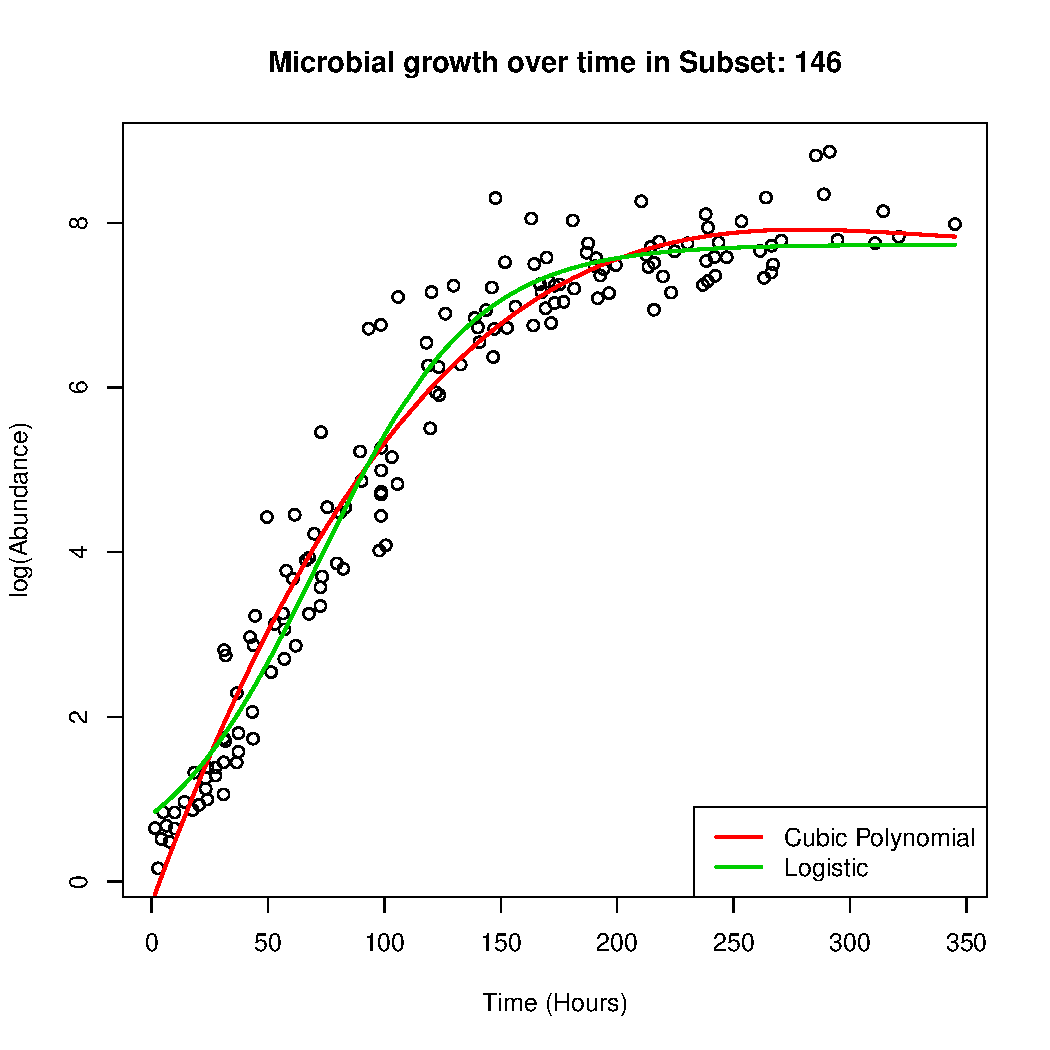
\includegraphics[scale=0.75]{../Plots/PlotID146.pdf}
    %TC:ignore
    \caption{Plot of a cubic polynomial and the logistic model fitted to one of the subsets within the dataset.}
    %TC:endignore
    \end{figure}

    \begin{figure}[H]
    \centering
    \includegraphics[scale=0.5]{../results/AIC.pdf}
    %TC:ignore
    \caption{AIC values of subsets}
    %TC:endignore
    \end{figure}

       \begin{figure}[H]
    \centering
    \includegraphics[scale=0.5]{../results/RSS.pdf}
    %TC:ignore
    \caption{RSS values for subsets}
    %TC:endignore
    \end{figure}

    \section*{Discussion}

	The aim of this study was to determine which of the models (Empirical or Mechanistic) best fit microbial growth data, and to compare model selection criteria. The logistic model had lower AIC values more often than the polynomial did across the subsets, suggesting that the logistic model has a higher likelihood of being an accurate fit. Additionally, the logistic model also had a lower RSS value the majority of the time. A lower RSS value for the likelihood model indicates that the logistic model accounts for more error than the polynomial. From these two selection criteria, the statistics suggest that the mechanistic logistic model both fits microbial growth curves better, explains more of the error, and is more likely to be a correct prediction than the polynomial model. Although these criteria suggest that  mechanistic model would be better for forecasting, larger sample sizes and repeated studies should be undertaken with a wider range of statistical analysis in order to further aid the future of model fitting. 


    \bibliographystyle{apalike}

    \bibliography{ReportBiblio}
\end{document}